\chapter{Evaluation}
\label{chap:experiments}

This chapter evaluates the methods developed throughout the thesis and
examines the central question motivating this work: \emph{how can a
learned world model be used to improve goal-conditioned control in
high-dimensional robotic manipulation tasks?}
The chapter proceeds from the most direct uses of the world model to the
more constrained ones. We begin by evaluating the model in isolation,
using model-predictive planning directly in latent space to establish
what can be achieved without policy learning
(\S\ref{sec:exp-cem-baseline}). We then test whether the world model can
replace the training environment for reinforcement learning
(\S\ref{sec:exp-wm-as-env}), before turning to MPC methods that keep the
model in a short-horizon proposal role. Finally, we evaluate the
hierarchical framework and compare the main approaches against the
strongest baselines across the benchmark suite.
Unless otherwise stated, all results are reported using the standard
OGBench evaluation protocol in the real MuJoCo environment. Additional
ablations and supporting experiments, including resolution studies,
TD-MPC2 comparisons, and partial world-model fine-tuning experiments,
are provided in the appendix.

% ---------------------------------------------------------------------
\section{Evaluation Setup}
\label{sec:exp-setup}

Experiments are conducted using the OGBench benchmark
\cite{ogbench_park2025}, which provides a suite of goal-conditioned
robotic manipulation tasks built on top of MuJoCo. The primary benchmark
used throughout this thesis is the
\texttt{cube-single-play} domain, consisting of five object-manipulation
tasks (\texttt{horizontal}, \texttt{vertical1},
\texttt{vertical2}, \texttt{diagonal1}, and
\texttt{diagonal2}). Observations are $224\times224$ RGB images and
actions are represented as five-step chunks of $5$-dimensional
end-effector commands.
World-model training and offline reinforcement-learning datasets are
constructed from the expert demonstrations distributed with OGBench.
For the offline-to-online experiments of
Chapters~\ref{chap:wm-env}-\ref{chap:mpc-distillation}, we additionally use the
\texttt{visual-cube-single-singletask-task1-v0} benchmark to enable
direct comparison with previously reported results
\cite{li2026reinforcementlearningactionchunking}.

The primary evaluation metric throughout this chapter is the
\emph{native OGBench success rate}. Policies are deployed in the real
MuJoCo simulator and a trial is counted as successful if the manipulated
cube finishes within $4$\,cm of the target pose. Results on the
multi-task benchmark are averaged over $50$ evaluation episodes per
task, while offline-to-online experiments use $250$ evaluation episodes
to reduce variance.

One exception is the CEM planning baseline in
\S\ref{sec:exp-cem-baseline}. Following the evaluation protocol used in
LeWM \cite{maes2026leworldmodelstableendtoendjointembedding},
we additionally report a \emph{latent-reaching} metric that measures
whether planning in latent space succeeds in reaching a target latent
state. This metric is useful for diagnosing world-model behaviour, but
it should not be interpreted as a measure of task completion and is not
used elsewhere in this chapter.

\subsection{World Model and Agent Instantiation}
\label{sec:exp-wm-instantiation}

We instantiate the latent action-conditioned world model from
Chapter~\ref{chap:foundations} using LeWM
\cite{maes2026leworldmodelstableendtoendjointembedding}. We use the
public implementation and train it on the same OGBench trajectories as
the downstream policies. The encoder $E_\xi$ is a ViT-Tiny model
\cite{dosovitskiy2021vit,touvron2021deit} that maps $224\times224$ RGB
observations to $192$-dimensional latent states. The predictor
$f_\psi$ is a Transformer that receives a short latent history and an
action chunk. Each world-model step corresponds to $h=5$ primitive
actions, so the predictor operates on $25$-dimensional action chunks
$c=(a_0,\ldots,a_4)\in\mathbb{R}^{25}$. The isotropy term in
Eq.~\eqref{eq:lewm-total-clean} is implemented as the Spectral Isotropy
Regulariser (SIGReg).

Unless stated otherwise, all experiments use the action-chunked Flow
Q-Learning (FQL) agent introduced in \S\ref{sec:fql-bg}, again with
chunk length $h=5$. The main optimisation constants are fixed across
experiments: discount factor $\gamma=0.99$, target-network Polyak
coefficient $\tau=0.005$, an ensemble of two critics averaged for value
estimation, and a one-step flow distillation coefficient
$\alpha=100$. The sparse-reward threshold in \S\ref{sec:wmep-setup} is
set to $\delta=2.0$, following the latent geometry analysis in
\S\ref{sec:wm-geometry}. Other implementation constants are listed in
Appendix~\ref{app:impl}.

% ---------------------------------------------------------------------
\section{World Model Diagnostics}
\label{sec:wm-quality}

The performance of all methods developed in this thesis ultimately
depends on the quality of the learned world model. Since the world
model is used both as a latent-state encoder and as a simulator for
imagined rollouts, any prediction error directly limits the quality of
the rewards, values, and subgoals produced by downstream algorithms.
Understanding these limitations is therefore essential for interpreting
the results presented in later chapters.

This section evaluates the world model from three complementary
perspectives. First, we measure how prediction error accumulates as
the rollout horizon increases (\S\ref{sec:wm-drift}), providing an
estimate of how far into the future the model can be trusted. Second,
we examine the geometry of the latent space induced by SIGReg
(\S\ref{sec:wm-geometry}), which underpins the distance-based rewards
used throughout this thesis. Finally, we compare world models trained
on different environments to assess how these properties generalise
across tasks (\S\ref{sec:wm-quality-envs}).

% \subsection{Pre-training}
% \label{sec:wm-pretrain}
% The predictor used throughout is the
% \texttt{version\_1} checkpoint, trained for $19$ epochs on the OGBench
% cube data ($224{\times}224$ images) with the LeWM loss of
% Eq.~\eqref{eq:lewm-total-clean}; validation prediction loss settles at
% $\approx 2.5 \times 10^{-3}$ and validation SIGReg at $\approx 1.4$.

\subsection{Prediction Drift over Rollout Horizon}
\label{sec:wm-drift}

A key property of any learned dynamics model is how prediction errors
accumulate over time. Even small inaccuracies compound when predicted
states are repeatedly fed back into the model, causing imagined
trajectories to gradually diverge from reality. We quantify this
effect using \emph{latent-space drift}.

Starting from a real trajectory, a short history of latent states and
actions is provided to the predictor $f_\psi$. The model is then rolled
forward for $\Delta$ future frames, and the predicted latent state
$\hat z_{t+\Delta}$ is compared against the latent representation of
the true observation at the same timestep. Drift is measured as the
Euclidean distance

\begin{equation}
\|\hat z_{t+\Delta} - z_{t+\Delta}\|_2.
\end{equation}
Table~\ref{tab:drift} reports the average drift measured on the
\texttt{visual-cube-single} environment. We focus on this environment
because it is the only OGBench task for which the original LeWM
authors provide pretrained checkpoints, making it the foundation of
all subsequent experiments.

\begin{table}[h]
\centering
\caption{Mean latent-space prediction drift as a function of rollout
horizon. Larger values indicate greater divergence between predicted
and ground-truth latent states.}
\label{tab:drift}
\begin{tabular}{lccccc}
\toprule
Prediction horizon $\Delta$ (frames) & 1 & 5 & 10 & 25 & 50 \\
\midrule
Mean drift $\|\hat z_{t+\Delta}-z_{t+\Delta}\|_2$
& 1.77 & 3.40 & 6.10 & 11.80 & 16.54 \\
\bottomrule
\end{tabular}
\end{table}

Several observations can be made from these results. First, prediction
error grows steadily with rollout horizon, as expected for an
autoregressive dynamics model. A single world-model step corresponds
to one action chunk of five environment frames. At this horizon the
average error is only $3.4$, indicating that short-horizon predictions
remain reasonably accurate.

More importantly, these values must be interpreted relative to the
scale of the latent space itself. Across the dataset, the average
distance between two latent states is approximately $7.4$. This
provides a useful reference point: once prediction drift becomes
comparable to this value, the model's uncertainty is on the same scale
as meaningful state differences.

This transition occurs after approximately two world-model steps
($10$ frames), where the average drift reaches $6.1$. Beyond this
point, prediction error is large enough that imagined states may be
closer to modelling artefacts than to the true future dynamics. At a
horizon of $25$--$50$ frames, the accumulated error substantially
exceeds the average latent-state separation, suggesting that long
open-loop rollouts should be treated with caution.

These findings have direct implications for the algorithms introduced
later in the thesis. Methods that rely only on short-horizon
predictions, such as reward shaping or local subgoal generation, can
operate within the model's reliable regime. In contrast, approaches
that perform long imagined rollouts must account for substantial model
bias. This limitation motivates several of the design choices made in
Chapter~\ref{chap:wm-as-subgoal}, where world-model predictions are used only for
short-horizon subgoal evaluation while value estimation remains
grounded in real data.

\subsection{Latent Geometry Analysis}
\label{sec:wm-geometry}

Many of the methods introduced in later chapters use Euclidean distance
in latent space as either a reward signal or a measure of progress
towards a goal. This only makes sense if distances have a consistent
interpretation throughout the latent space. For example, if some states
naturally had very large latent norms while others had very small norms,
then the same distance threshold could correspond to very different
amounts of semantic change depending on where the agent was located.
Any reward based on latent distance would therefore require extensive
per-task tuning.

SIGReg was introduced during world-model training specifically to avoid
this issue. Rather than allowing latent representations to spread
unevenly through the embedding space, it encourages the latent
distribution to remain approximately isotropic, meaning that all
directions and regions of the space have a similar scale. In practice,
this implies that latent norms should be concentrated around a common
value rather than varying dramatically across states.

Figure~\ref{fig:latent-norms} shows the distribution of latent norms for
goal states drawn from outside the training set. The goal latent norms lie on a
similar-radius shell rather than occupying regions with very different
absolute scales. This matters because Euclidean thresholds would be hard
to interpret if some goals naturally had much larger norms than others:
distance would then be dominated by where the goal sits relative to the
origin rather than by local state similarity. Throughout this thesis we
use a fixed success threshold $\delta_d = 2.0$ in latent space, so this
plot is a sanity check that a single threshold is at least geometrically
well conditioned. The later CEM baseline tests the separate question of
whether latent proximity is sufficient for native task success.

\begin{figure}[h]
\centering
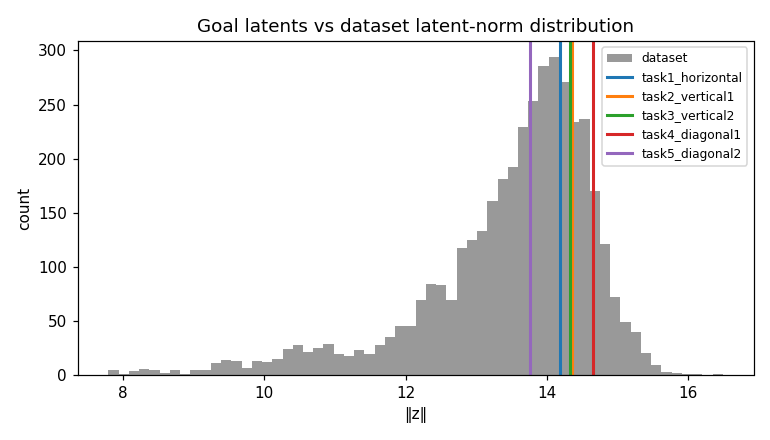
\includegraphics[width=0.55\linewidth]{figures/goal_norms_ood.png}
\caption{Distribution of latent norms for out-of-distribution goal
states. The mass is concentrated around a single radius rather than
split across widely separated norm scales. This supports using one
latent-distance threshold across goals, but does not by itself imply
that latent proximity is equivalent to task completion.}
\label{fig:latent-norms}
\end{figure}

% ---------------------------------------------------------------------
\subsection{World Model Diagnostics Across Environments}
\label{sec:wm-quality-envs}

The previous sections focused on the
\texttt{visual-cube-single-v0} environment because it is the only
OGBench task for which pretrained LeWM weights are publicly available.
To evaluate whether the conclusions generalise beyond this setting, we
also train world models for two additional OGBench environments:

\begin{itemize}
    \item \texttt{visual-scene-play-v0}, a tabletop manipulation
    environment containing multiple objects and button-press tasks;
    \item \texttt{visual-puzzle-3x3-play-v0}, a sliding-tile puzzle in
    which progress depends on discrete button activations.
\end{itemize}

All three world models are trained using the same architecture and
training procedure: a ViT-Tiny encoder, Transformer predictor,
SIGReg regularisation, and $224\times224$ image observations. The
resulting models are then evaluated using the same diagnostics
introduced above.

\paragraph{Predictor drift.}

Table~\ref{tab:drift-multienv} reports predictor drift as a function of
rollout horizon for all three environments. Recall that drift measures
the latent-space error between a predicted future state and the
corresponding ground-truth encoded state. Smaller values therefore
indicate a more accurate dynamics model. Several trends are immediately visible.

First, the scene environment is substantially easier to model than the
cube environment. Drift remains low even at longer horizons, suggesting
that imagined rollouts remain reliable for several world-model steps.
Second, the puzzle environment is dramatically more difficult. After a
single world-model step ($\Delta=5$ frames), the average prediction
error already exceeds $8.8$, which is larger than the average distance
between many semantically distinct states in the cube environment.
Errors then continue to grow with rollout horizon.
We believe this difference is a consequence of the underlying task
dynamics. The cube and scene environments are dominated by smooth,
continuous object motion, which is well suited to latent prediction.
The puzzle environment, by contrast, contains discrete button-flip
events that abruptly change the state of the puzzle. Such transitions
are difficult for a continuous predictor to anticipate accurately,
leading to significantly larger rollout errors.

\begin{table}[h]
\centering
\caption{Predictor drift
$\|\hat{z}_{t+\Delta}-z_{t+\Delta}\|_2$
across three environments. Lower values indicate more accurate
long-horizon predictions.}
\label{tab:drift-multienv}
\begin{tabular}{lcccc}
\toprule
Environment & $\Delta=5$ & $\Delta=10$ & $\Delta=25$ & $\Delta=50$ \\
\midrule
cube-single & 3.40 & 6.10 & 11.80 & 16.54 \\
scene       & 1.23 & 2.20 & 4.92 & 7.76 \\
puzzle-3x3  & 8.88 & 13.53 & 17.01 & 19.03 \\
\bottomrule
\end{tabular}
\end{table}

Figure~\ref{fig:drift-multienv} visualises the same results. The key
observation is that rollout accuracy degrades at very different rates
across environments. This suggests that downstream planning methods
should not be expected to benefit equally from a world model even when
the architecture and training procedure are identical.

\begin{figure}[h]
\centering
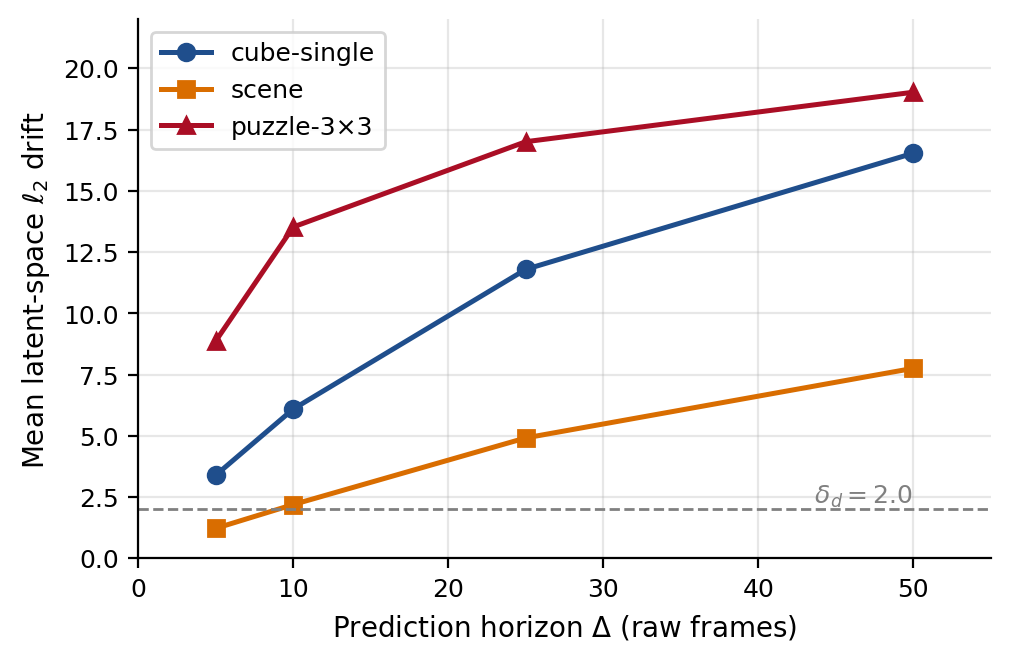
\includegraphics[width=0.68\linewidth]{figures/multi_env_predictor_drift.png}
\caption{Predictor drift as a function of rollout horizon. Lower curves
indicate more accurate imagined trajectories. The scene environment
remains predictable over substantially longer horizons than the cube or
puzzle environments.}
\label{fig:drift-multienv}
\end{figure}

\paragraph{Action conditioning.}

Predictor accuracy alone is not sufficient for planning. A planner must
also be able to influence the future state through its choice of
actions. A world model that accurately predicts the future but largely
ignores its action inputs would be unsuitable for model-based control.

To measure this property, we compare predictions generated using the
true action sequence with predictions generated using randomly shuffled
actions. If shuffling the actions causes prediction quality to
deteriorate substantially, then the predictor must be using the action
signal. Conversely, if the prediction error remains almost unchanged,
the predictor is largely insensitive to the chosen actions.

Figure~\ref{fig:action-cond} reports the resulting
action-conditioning ratio. Larger ratios indicate stronger dependence
on the action sequence and therefore greater controllability.
The cube model exhibits extremely strong action conditioning: replacing
the correct actions with shuffled actions increases prediction error by
a factor of approximately $8\times$. This indicates that the model has
learned a strong relationship between actions and future states, making
it well suited for planning.
The scene model remains action-conditioned, but much less strongly
($1.4\times$). The predictor responds to control inputs, although the
effect is relatively modest.
The puzzle model shows almost no action sensitivity
($1.1\times$). In practice, this means that imagined futures are nearly
the same regardless of which actions are supplied. Such a model may
still reconstruct the average behaviour observed in the dataset, but it
provides little useful information for selecting actions.

\begin{figure}[h]
\centering
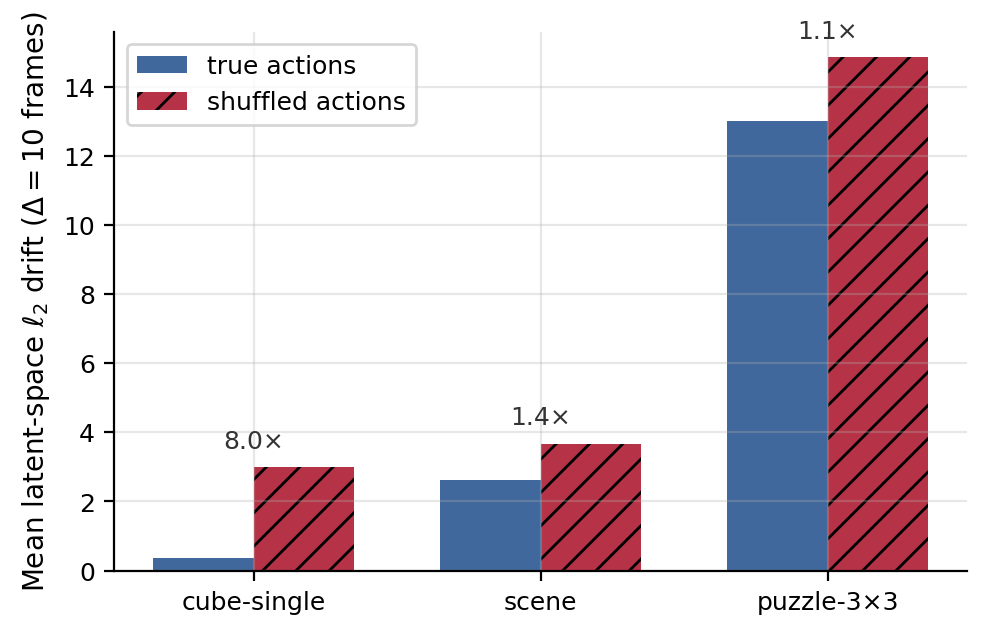
\includegraphics[width=0.65\linewidth]{figures/action_conditioning.png}
\caption{Action-conditioning diagnostic. Larger ratios indicate that
the predictor strongly depends on its action inputs, which is a
prerequisite for effective model-based planning.}
\label{fig:action-cond}
\end{figure}

\paragraph{Latent-space quality.}

Finally, we verify that the latent geometry remains well behaved across
all environments. Table~\ref{tab:norms-multienv} reports the mean and
standard deviation of latent norms for states drawn from each dataset.
The most important observation is not the exact numerical value of the
norms, but their consistency. Across all environments, latent vectors
occupy approximately the same scale and exhibit relatively small
variance. This suggests that SIGReg is successfully enforcing a
well-conditioned latent geometry regardless of task.
In addition, all goal states remain clearly separated from one another
in latent space, and no dataset state falls within the success
threshold of an incorrect goal. Consequently, the distance-based reward
functions used throughout this thesis remain meaningful without any
environment-specific recalibration.

\begin{table}[h]
\centering
\caption{Latent norm statistics across environments. Similar norm
scales indicate that SIGReg produces a consistent latent geometry even
when the underlying tasks differ substantially.}
\label{tab:norms-multienv}
\begin{tabular}{lrrl}
\toprule
Environment & Dataset mean & Dataset std & Goal mean \\
\midrule
cube-single & 13.47 & 1.26 & 14.28 \\
scene       & 13.92 & 0.70 & 13.53 \\
puzzle-3x3  & 13.80 & 0.57 & 13.97 \\
\bottomrule
\end{tabular}
\end{table}

Taken together, these diagnostics suggest that latent-space quality is
not the limiting factor for downstream performance. All three models
produce well-structured latent representations. Instead, the critical
difference lies in the interaction between prediction accuracy and
action conditioning. As we show in
\S\ref{sec:exp-generalisation}, these two properties are much more
predictive of whether model-based planning methods succeed than either
raw latent geometry or reconstruction quality alone.

% ---------------------------------------------------------------------
\section{Latent-Space Planning Baseline}
\label{sec:exp-cem-baseline}

Before evaluating learned policies, we first ask how far the frozen
world model can be pushed on its own. To answer this, we use the same
Cross-Entropy Method (CEM) \cite{Rubinstein1999} planning procedure employed in the original
LeWM work. Rather than learning a policy, CEM directly
optimises sequences of actions against the world-model dynamics,
selecting the action sequence that minimises the latent-space distance
to a target goal state.
This experiment represents the strongest possible \emph{world-model
only} baseline: planning is performed directly in the latent space used
to train the predictor, without any approximation introduced by policy
learning or value estimation.

\begin{table}[h]
\centering
\caption{CEM planning directly in the $224{\times}224$ LeWM latent
space (\texttt{terminate\_at\_goal}, $50$ episodes).
\emph{Latent-reach} is the in-distribution training-time diagnostic;
\emph{native task success} is the OGBench block-pose criterion --- the
metric every subsequent table is measured against. The contrast is
the central observation that frames the rest of this chapter.}
\label{tab:cem-baseline}
\begin{tabular}{lc}
\toprule
Setting & Value \\
\midrule
Plan / receding horizon      & 5 / 5 \\
Action block                 & 5 \\
CEM samples $\times$ iters   & $300 \times 30$ \\
CEM elite (top-$k$)          & 30 \\
\midrule
Latent-reach rate            & $72.0\%$ \\
\textbf{Native task success} & \textbf{$0.0\%$} \\
\bottomrule
\end{tabular}
\end{table}

The result (Table~\ref{tab:cem-baseline}) reveals an important limitation of the learned latent space.
While the planner successfully reaches the target latent state in
approximately $72\%$ of episodes, it fails to solve a single cube
manipulation task when evaluated in the real MuJoCo environment.
This discrepancy demonstrates that latent-space proximity and task
completion are not equivalent objectives. The world model has learned a
representation in which nearby latent states are predictive of future
observations, but reaching a target embedding does not necessarily imply
that the physical object has reached the desired configuration. In other
words, the latent geometry is useful for prediction but is not, by
itself, a sufficient control objective.
The remaining experiments therefore use latent rollouts only when their
outcomes are judged by a critic or policy trained on real task data.

% ---------------------------------------------------------------------
\section{World Model as Environment Results}
\label{sec:exp-wm-as-env}

Chapter~\ref{chap:wm-env} introduced the variants that use LeWM as a
surrogate environment for online fine-tuning. This section reports their
real-environment performance and the diagnostic comparisons needed to
interpret the failures. Across all variants tested, synthetic
world-model interaction fails to improve the offline policy.

\subsection{Offline-to-Online Reinforcement Learning inside World Model}
\label{sec:exp-oo-wm-env}

Figure~\ref{fig:wm-env-curves} shows the training curves for the
principal variants introduced in Chapter~\ref{chap:wm-env}, while
Table~\ref{tab:owm-summary} reports their final performance when
evaluated in the real MuJoCo environment.
A consistent pattern emerges across all experiments: none of the
world-model-based training procedures improve upon the offline policy
from which they start. The control row shows that the same latent
representation can support online improvement under true dynamics, so
the degradation is specific to using the predictor as the transition
model.

\begin{figure}[h]
\centering
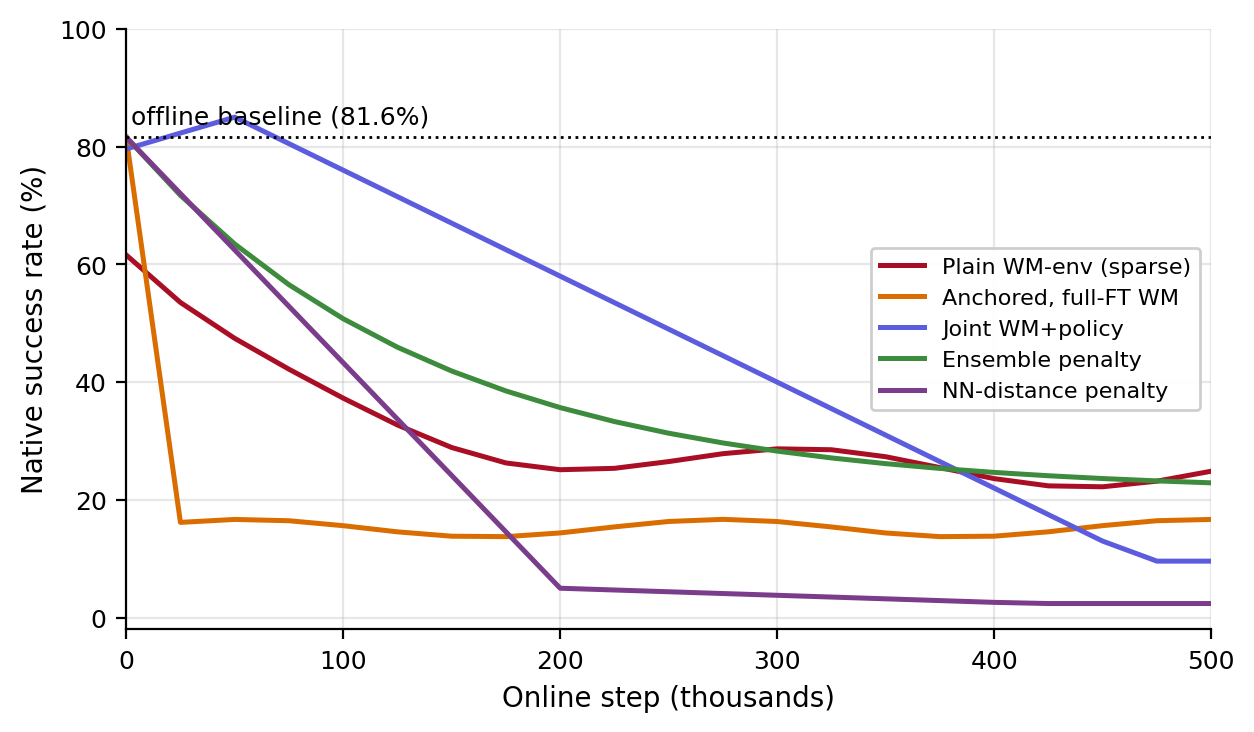
\includegraphics[width=0.85\linewidth]{figures/wm_env_training_curves.png}
\caption{Training-time success rate during world-model fine-tuning on
\texttt{visual-cube-single-singletask-task1-v0}. The horizontal dashed
line indicates the performance of the initial offline policy
($81.6\%$). All variants remain below this baseline throughout training,
demonstrating that online reinforcement learning inside the learned
world model does not translate into improved real-environment
performance.}
\label{fig:wm-env-curves}
\end{figure}

\begin{table}[h]
\centering
\caption{Final real-environment performance after the online phase for
world-model-as-environment approaches on
\texttt{visual-cube-single-singletask-task1-v0}. The main offline
starting checkpoint has $81.6\%$ success; the jointly trained policy
starts from $79.6\%$. The table reports the final online result only,
measured over $250$ evaluation episodes, except for the real-dynamics
control, which was evaluated over $50$ episodes. Multi-run settings
report mean $\pm$ standard deviation; single-run diagnostics are marked
with $1$ run.}
\label{tab:owm-summary}
\begin{tabular}{lcr}
\toprule
Variant & Runs & Final SR (\%) \\
\midrule
\multicolumn{3}{l}{\emph{Real-dynamics control}} \\
Latent observations, real dynamics & 1 & \textbf{100.0} \\
\midrule
\multicolumn{3}{l}{\emph{Direct WM interaction}} \\
Sparse reward & 3 & $24.5 \pm 5.1$ \\
Anchored, sparse reward & 3 & $17.2 \pm 4.9$ \\
Anchored, dense reward & 3 & $15.2 \pm 2.3$ \\
\midrule
\multicolumn{3}{l}{\emph{Predictor adaptation and component swap}} \\
Joint predictor--policy training & 1 & 9.6 \\
\quad Base policy + jointly trained predictor & 1 & 7.2 \\
\quad Jointly trained policy + base predictor & 1 & 30.0 \\
\midrule
\multicolumn{3}{l}{\emph{Uncertainty-penalised rewards}} \\
Ensemble uncertainty penalty & 1 & 21.2 \\
Nearest-neighbour regularisation & 1 & 2.4 \\
\bottomrule
\end{tabular}
\end{table}

The most striking observation is the contrast with the control
experiment. When the policy is trained online using the real
environment while retaining the same latent observation space,
performance improves from $81.6\%$ to perfect success. The limitation
therefore does not lie in the policy architecture or the latent
representation itself; it lies in treating the learned predictor as a
drop-in replacement for the environment.

The direct world-model interaction and anchored rows show that shortening
imagined rollouts is not enough to recover performance. Sparse
world-model interaction ends at $24.5 \pm 5.1\%$, while anchored sparse
and dense variants reach only $17.2 \pm 4.9\%$ and $15.2\%$. This
supports the interpretation from Chapter~\ref{chap:wm-env}: anchoring
can limit the most extreme predictor drift, but the replay buffer still
contains model-generated transitions whose errors enter value learning.
The uncertainty-penalised rows tell a similar story. Ensemble
disagreement improves only modestly to $21.2\%$, while nearest-neighbour
regularisation falls to $2.4\%$, consistent with the concern that
distance from the offline dataset is not the same as prediction error
and can penalise task-relevant but sparsely represented states.

\paragraph{Joint predictor--policy component swap.}
\label{sec:eval-joint}
The diagnostic rows associated with joint predictor--policy training
provide further insight. Replacing the jointly trained policy with the
original offline policy while keeping the jointly trained predictor
reduces performance to only $7.2\%$. Conversely, replacing the
jointly trained predictor with the original frozen predictor raises
performance to $30.0\%$. This points more strongly to the predictor
than to the policy as the source of the collapse: modifying the world
model during training appears to introduce errors that are subsequently
exploited by the reinforcement-learning objective. Together, these
results support the negative case developed in Chapter~\ref{chap:wm-env}:
LeWM is useful as a representation and short-horizon predictor, but not
as an unrestricted training environment.

% ---------------------------------------------------------------------

% \paragraph{Flow-DPO (CPU test only).}
% A contrastive preference update (Flow-DPO, \S\ref{sec:phase2-dpo})
% that selects the highest-scoring WM-rollout candidate as ``winner''
% and the lowest as ``loser'' was validated on CPU only. The
% WM-rollout metric $V_{\mathrm{roll}}$ fell from $-34.4$ to $-46.3$
% in $20$ steps --- the sharpest degradation of any approach tested
% --- owing to high gradient correlation between winner and loser in
% the Phase-1 flow's concentrated distribution. Flow-DPO was not run
% on the cluster.

% ---------------------------------------------------------------------
\section{World Model as Planner Results}
\label{sec:exp-mpc}

Chapter~\ref{chap:wm-planner} introduced the inference-time planners.
Here we evaluate them on the frozen offline policy. The pattern is
simple: short-horizon planning improves action selection, while longer
rollouts lose reliability as world-model error accumulates.

\subsection{Scoring Functions}
\label{sec:exp-scoring}

We use the three scoring rules defined in
Chapter~\ref{chap:wm-planner}: terminal critic scoring (Q-term),
trajectory-wide critic scoring (Q-all), and latent-distance shaping plus
terminal critic scoring (Dense+Q). Unless otherwise stated we use
Q-term. Q-all becomes useful later, after the critic has been trained on
planner-shaped actions.

\subsection{Inference-Time MPC on a Frozen Policy}
\label{sec:exp-mpc-frozen}

We first evaluate planning without any parameter updates. Starting from
the $81.6\%$ offline checkpoint, BoN-MPC samples $N=32$ action chunks
and ranks their short rollouts. Grad-MPC then adds five gradient-ascent
steps through the differentiable world model. Any improvement therefore
comes from test-time computation alone.

\begin{table}[h]
\centering
\caption{Best-of-$N$ MPC applied to a frozen offline policy.
Performance is measured in the real environment over 250 evaluation
episodes. The offline policy achieves 81.6\% success without planning.}
\label{tab:mpc-bon}
\begin{tabular}{l c l r}
\toprule
Method & Horizon $H$ & Trajectory Score & Success (\%) \\
\midrule
BoN-MPC                 & 1 & Q-term    & \textbf{88.0} \\
BoN-MPC                 & 1 & dense$+$Q & 87.2 \\
BoN-MPC                 & 2 & Q-term    & 83.6 \\
BoN-MPC                 & 2 & dense$+$Q & 81.6 \\
BoN-MPC                 & 3 & Q-term    & 80.4 \\
BoN-MPC                 & 3 & dense$+$Q & 79.2 \\
\bottomrule
\end{tabular}
\end{table}

Table~\ref{tab:mpc-bon} demonstrates that planning provides a
meaningful improvement even when all learned parameters remain frozen.
The best configuration reaches $88.0\%$ success, improving upon the
$81.6\%$ offline baseline by $6.4$ percentage points.
More interesting than the absolute gain is the effect of planning
horizon. Performance peaks at a single world-model step and then
degrades as the horizon increases. By $H=3$, performance has fallen
below the offline baseline.
This behaviour mirrors the world-model drift analysis of
\S\ref{sec:wm-drift}. Small prediction errors accumulate across the
rollout, causing the terminal state evaluated by the critic to become
progressively less reliable. The planner therefore receives the most
useful signal when the world model is used only for short-range
lookahead.

\begin{table}[h]
\centering
\caption{Gradient-refined MPC applied to the same frozen offline policy.
Starting from the best BoN candidate, actions are refined using five
gradient-ascent steps through the world model.}
\label{tab:mpc-grad}
\begin{tabular}{l c l r}
\toprule
Method & $H$ & Scoring & SR (\%) \\
\midrule
Grad-MPC      & 1 & Q-term    & 88.8 \\
Grad-MPC      & 2 & Q-term    & \textbf{90.0} \\
Grad-MPC      & 3 & Q-term & 88.8 \\
\bottomrule
\end{tabular}
\end{table}

Grad-MPC further improves performance, reaching $90.0\%$ success at
$H=2$. Relative to the offline baseline this corresponds to an
absolute gain of $8.4$ percentage points, achieved without any
additional policy training.
The improvement suggests that the world model contains useful local
gradient information even when its long-horizon predictions are
imperfect. Rather than relying entirely on sampled candidates,
Grad-MPC is able to exploit the differentiable structure of the
predictor to refine actions toward higher-value outcomes.

\paragraph{Why does Q-term outperform Dense+Q?}

Across both MPC variants, the strongest results are obtained using
Q-term scoring. Incorporating latent-distance rewards consistently
reduces performance.
This result is important because it links directly back to the CEM
baseline of \S\ref{sec:exp-cem-baseline}. There we observed that
optimising purely for latent proximity produced a $72.0\%$
latent-reach rate but $0.0\%$ task success. The latent geometry learned
by the world model therefore does not perfectly align with task
completion in the real environment.
The critic provides a way around this problem. Unlike latent distance,
the critic was trained using real task rewards and therefore encodes
information about actual task progress. Q-term effectively uses the
world model only to propose future states while delegating the final
evaluation to a function grounded in real experience.
The results suggest that the limitation is not the imagined rollout
itself, but rather the objective used to evaluate it.

\subsection{FMQ on the Frozen Offline Critic}
\label{sec:exp-fmq-base}

FMQ replaces iterative gradient optimisation with a single
normalised gradient step constrained by a trust-region radius
$\eta$. Intuitively, FMQ attempts to move actions toward regions of
higher critic value while remaining close to the behaviour policy.
Table~\ref{tab:mpc-fmq-basepolicy} evaluates FMQ using the original
offline critic.

\begin{table}[h]
\centering
\caption{FMQ planning using the original offline critic.
The critic was trained only on dataset actions and has not been
exposed to FMQ-optimised actions.}
\label{tab:mpc-fmq-basepolicy}
\begin{tabular}{c l c r}
\toprule
$H$ & Scoring & $\eta$ & SR (\%) \\
\midrule
2 & Q-all  & 0.10 & \textbf{90.0} \\
2 & Q-all  & 0.30 & 57.2 \\
2 & Q-all  & 0.50 & 25.6 \\
1 & Q-all  & 0.30 & 60.0 \\
2 & Q-term & 0.30 & 58.8 \\
1 & Q-term & 0.30 & 61.2 \\
\bottomrule
\end{tabular}
\end{table}

The best configuration reaches $90.0\%$ success at $\eta=0.1$,
matching the strongest Grad-MPC result. However, performance
deteriorates rapidly as the trust-region radius increases.
At $\eta=0.3$, success falls to approximately $60\%$, and by
$\eta=0.5$ it drops below $30\%$. This behaviour indicates that the
failure is not caused by FMQ itself but by critic extrapolation.
The offline critic was trained exclusively on actions produced by the
behaviour policy. Large FMQ updates move candidate actions into
regions of the action space where the critic has little training data.
Although the critic may assign high values to these actions, those
estimates are no longer reliable, causing the planner to optimise
against inaccuracies in the value function.
This observation motivates the interleaved training procedure of
the next section. By retraining the critic on FMQ-generated actions,
the region of reliable optimisation can be expanded substantially,
allowing larger planning improvements without critic collapse.

% ---------------------------------------------------------------------
\section{World Model as Data Generator Results}

This section evaluates three ways of turning short-horizon planning into
training data. The first uses the planner only to relabel actions for
offline states. The second generates full imagined transitions during an
online fine-tuning phase inside the world model. The third removes the
online loop entirely by generating a fixed synthetic corpus before
training.
The key distinction is whether generated data remains coupled to the
current actor and critic. Interleaved action relabelling keeps this loop
tight: planner-generated actions are produced from the current networks
and can be folded back into actor and critic updates. Online
world-model fine-tuning keeps the planner in the loop but asks a harder
question, namely whether imagined successor states can safely enter
replay. Static dataset generation breaks the loop, so the learner must
extract value from trajectories produced by a different fixed policy.
The results below show that generated data is useful mainly in the
coupled settings; as a one-shot replacement for real offline data, it is
substantially weaker.

\subsection{Interleaved Learning from Grad-MPC Actions}
\label{sec:exp-mpc-interleaved-grad}

We first evaluate planner-generated action targets. In this setting the
world model is not used to create new states or rewards. Instead,
Grad-MPC is applied to offline latent states to produce improved action
chunks, which are then used as additional training targets.
The interleaved training procedure of \S\ref{sec:mpcd-interleaved}
periodically runs Grad-MPC on a fresh batch of offline latent states and
stores the resulting labelled pairs
$(z,\mathbf{a}^{\mathrm{MPC}})$. In the experiments below this
relabel step is performed every $25$k gradient updates, using
Grad-MPC with $K=5$.
We compare two ways of using these labels. In the actor-only setting,
the labels are used for an additional policy update and the critic
continues to train on the original offline actions. In the critic-update
setting, a fraction of each training batch is replaced by MPC-labelled
actions, so the critic is also trained on the planner's action
distribution. This distinction tests whether the actor can benefit from
planner labels when the critic has never been calibrated on the same
actions.

\begin{table}[h]
\centering
\caption{Interleaved training with Grad-MPC labels. All runs start from
the $81.6\%$ offline checkpoint and train for $5\times 10^5$ gradient
steps. \emph{0-S SR} evaluates the trained actor zero-shot, without
world-model planning at test time ($\mathrm{BoN}\,N=4$). \emph{MPC SR} reapplies
Grad-MPC ($N=32$, $H=2$, $K=5$) on top of the final actor. The critic
update column indicates whether MPC-labelled actions are also used in
critic batches.}
\label{tab:mpc-interleaved-grad}
\begin{tabular}{lcrr}
\toprule
Planner label config & Critic update & 0-S SR (\%) & MPC SR (\%) \\
\midrule
$N=8,\ H=1,\ K=3$  & No & 83.6 & 86.8 \\
$N=8,\ H=1,\ K=3$  & Yes, $p=0.3$ & 81.6 & 91.2 \\
$N=32,\ H=2,\ K=5$ & No & 84.0 & 85.6 \\
$N=32,\ H=2,\ K=5$ & Yes, $p=0.3$ & 82.8 & \textbf{92.4} \\
\bottomrule
\end{tabular}
\end{table}

Table~\ref{tab:mpc-interleaved-grad} shows that the critic-update
setting is consistently better under MPC evaluation. Although the
standalone actor does not improve dramatically, exposing the critic to
planner-shaped actions keeps the actor and critic calibrated to the same
local policy-improvement step. The comparison suggests that
planner-generated actions are most useful when the critic is trained on
the same action distribution as the actor.

\subsection{Interleaved Learning from FMQ Actions}
\label{sec:exp-mpc-fmq-distil}

We next replace Grad-MPC with the FMQ label generator introduced in
\S\ref{sec:mpcd-interleaved}. Each relabelling pass uses
$\eta_{\mathrm{train}}=0.1$, $H=2$, and $N=32$, and mixes the resulting
actions into the main FQL batch with probability $p=0.3$. This tests
whether training on FMQ-shaped actions resolves the narrow
trust-region sensitivity observed with the frozen critic in
\S\ref{sec:exp-fmq-base}.

\paragraph{Effect of the relabelling interval.}
Figure~\ref{fig:fmq-distil-curves} and
Table~\ref{tab:mpc-relabel-sweep} compare two relabelling schedules.
The medium schedule relabels every $25$k steps, while the slow schedule
relabels every $50$k steps. This sweep tests the trade-off between
targets that change too quickly and labels that become stale.

\begin{figure}[h]
\centering
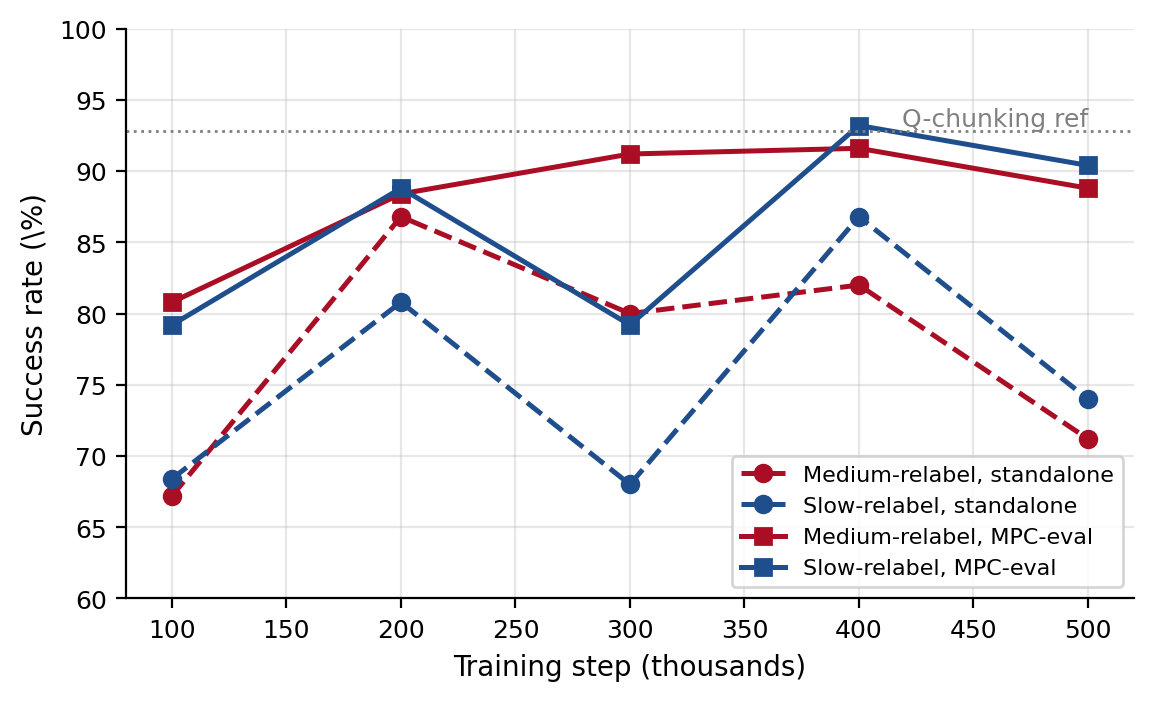
\includegraphics[width=0.85\linewidth]{figures/fmq_distil_curves.png}
\caption{Training curves for FMQ-label interleaved training.
Dashed lines show standalone success rate without world-model planning
at test time. Solid lines show MPC success rate after applying
Grad-MPC ($N=32$, $H=2$, $K=5$) to the trained actor. The slow
relabel schedule produces a cleaner peak of $93.2\%$ MPC success
at $400$k steps. The dotted line marks the Q-chunking reference
($92.8\%$).}
\label{fig:fmq-distil-curves}
\end{figure}

\begin{table}[h]
\centering
\caption{Effect of the FMQ relabelling interval during interleaved
MPC-based training. All runs use FMQ labels with
$\eta_{\mathrm{train}}=0.1$, $H=2$, $N=32$, and critic-update
probability $p=0.3$. Standalone SR evaluates the actor without the
world model. MPC SR applies Grad-MPC
($N=32$, $H=2$, $K=5$, Q-term) on top of the actor at each checkpoint.}
\label{tab:mpc-relabel-sweep}
\begin{tabular}{llrrrrr}
\toprule
Evaluation & Relabel Interval & 100k & 200k & 300k & 400k & 500k \\
\midrule
Standalone SR (\%) -- FMQ labels & 25k & 67.2 & \textbf{86.8} & 80.0 & 82.0 & 71.2 \\
Standalone SR (\%) -- FMQ labels & 50k & 68.4 & 80.8 & 68.0 & \textbf{86.8} & 74.0 \\
\midrule
MPC SR (\%) -- FMQ labels & 25k & 80.8 & 88.4 & 91.2 & 91.6 & 88.8 \\
MPC SR (\%) -- FMQ labels & 50k & 79.2 & 88.8 & 79.2 & \textbf{93.2} & 90.4 \\
\bottomrule
\end{tabular}
\end{table}

The medium relabelling schedule improves quickly but is less stable:
standalone success rises to $86.8\%$ at $200$k, then falls to
$71.2\%$ by $500$k. This suggests that frequent relabelling creates a
moving-target effect, where the actor and critic repeatedly adapt to
labels produced by a rapidly changing optimisation landscape.
The slow relabelling schedule is less aggressive but produces the best
checkpoint. At $400$k steps it reaches $86.8\%$ standalone success and
$93.2\%$ under MPC evaluation. This checkpoint is then used for the FMQ inference sweep below.
A full sweep over learning rate, buffer size, mix ratio, relabelling
interval, and trust-region radius, together with the early
high-frequency-relabel variants, is reported in
Appendix~\ref{app:oo-sweeps}.

\subsection{FMQ Inference after Learning from Generated Actions}
\label{sec:exp-fmq-distil-inf}

We now test whether FMQ-labelled training improves inference-time FMQ
planning. The key question is whether a critic trained on FMQ-shaped
actions remains reliable over a wider range of trust-region radii
$\eta$.
Table~\ref{tab:mpc-fmq-distilled} confirms this hypothesis. Unlike the
base critic in Table~\ref{tab:mpc-fmq-basepolicy}, which collapsed
rapidly for large $\eta$, the FMQ-trained critic remains above
$94.0\%$ success for $\eta \in [0.01,0.05]$ and reaches a peak success
rate of $96.0\%$ at both $\eta=0.02$ and $\eta=0.03$.

\begin{table}[h]
\centering
\caption{Inference-time planning on the FMQ-trained actor. The actor
is the $400$k checkpoint from the slow-relabel FMQ-trained run.
FMQ uses Q-all scoring unless stated otherwise. The broad high-performing
range of $\eta$ shows that the critic has become calibrated for
FMQ-shaped actions.}
\label{tab:mpc-fmq-distilled}
\begin{tabular}{lllr}
\toprule
Inference Method & Trajectory Score & Configuration & Success (\%) \\
\midrule
FMQ & Q-all  & $\eta = 0.01$ & 94.8 \\
FMQ & Q-all  & $\eta = 0.02$ & \textbf{96.0} \\
FMQ & Q-all  & $\eta = 0.03$ & \textbf{96.0} \\
FMQ & Q-all  & $\eta = 0.05$ & 94.0 \\
FMQ & Q-all  & $\eta = 0.10$ & 90.8 \\
FMQ & Q-all  & $\eta = 0.20$ & 80.8 \\
FMQ & Q-term & $\eta = 0.05$ & 93.6 \\
\midrule
Grad-MPC & Q-term & $K = 5$  & 93.2 \\
Grad-MPC & Q-term & $K = 8$  & \textbf{96.0} \\
Grad-MPC & Q-term & $K = 10$ & 90.8 \\
\midrule
Standalone trained actor & -- & $\mathrm{BoN}\,N=4$ & 86.8 \\
Q-chunking reference & -- & Published baseline & 92.8 \\
\bottomrule
\end{tabular}
\end{table}

This setting reaches a $96.0\%$ success rate, exceeding the Q-chunking
reference by $3.2$ percentage points and improving substantially over
the original $81.6\%$ offline checkpoint. Importantly, this improvement
does not come from using the world model as a training environment.
Instead, the world model is used in a controlled way: first to generate
planner-improved action labels, and then at inference time to make
short, trust-region-constrained action refinements.

\paragraph{Why Q-all works after FMQ-based training.}
The FMQ-trained rows use Q-all scoring by default. This differs from
the earlier frozen-policy MPC experiments, where Q-term was more robust.
The reason is that the critic has now been trained on FMQ-shaped actions
throughout the rollout, not only at the terminal state. Intermediate
critic values are therefore better calibrated, allowing Q-all to extract
more information from each imagined trajectory.
This isolates the role of critic calibration. Q-all is unreliable when
the critic has only seen dataset actions, but becomes useful once
interleaved training brings FMQ-modified actions into the critic's
training distribution.

\subsection{Actor Fine-Tuning with World-Model Transitions}
\label{sec:exp-mpc-online-wm}

The experiments above generate improved action targets but no new
state transitions. We next evaluate the online-in-WM procedure of
\S\ref{sec:mpcd-online-wm}, where FMQ-MPC rollouts inside the frozen
world model append imagined transitions to a replay buffer seeded with
offline data. We compare actor+critic updates against an actor-only
variant with the critic frozen, isolating whether imagined successors
can safely enter value learning.

\begin{table}[h]
\centering
\caption{Online fine-tuning with world-model-generated transitions on
\texttt{visual-cube-single-singletask-task1-v0}. All online runs use
FMQ-MPC inside the world model for $500{,}000$ steps
($N=32$, $H=2$, $\eta=0.02$, Q-all scoring). Success rate is measured
without a planner at test time over $250$ episodes, reported as mean
$\pm$ standard deviation over three seeds.}
\label{tab:mpc-online-e2}
\begin{tabular}{lcc}
\toprule
Method & Final Success (\%) & Peak Success (\%) \\
\midrule
Offline FQL checkpoint & 81.6 & 88.0 \\
Actor+critic update on imagined data & 30.7 $\pm$ 20.8 & 89.5 $\pm$ 0.7 \\
Actor-only update with frozen critic & \textbf{90.7 $\pm$ 0.8} & \textbf{94.8 $\pm$ 0.7} \\
\midrule
Frozen-critic checkpoint + FMQ-MPC at test time & -- & 93.2 $\pm$ 0.7 \\
\bottomrule
\end{tabular}
\end{table}

Table~\ref{tab:mpc-online-e2} and Figure~\ref{fig:online-in-wm-curves} show a sharp contrast between the two
training strategies. When the critic is updated on imagined transitions,
training initially improves but later collapses, ending at only
$30.7 \pm 20.8\%$ success. This mirrors the failure mode observed in
the world-model-as-environment experiments: once the critic is trained
on model-generated targets, value estimates become corrupted by
prediction error and, in the single-task setting, by the mismatch
between offline and generated reward scales. The actor then begins to
exploit those inaccuracies.
Freezing the critic prevents this collapse. The actor-only variant
improves smoothly, reaching a peak success rate of
$94.8 \pm 0.7\%$ and a final success rate of $90.7 \pm 0.8\%$. This is a
substantial improvement over the offline starting point, demonstrating
that imagined transitions can be useful when they are used as
policy-improvement data rather than as targets for critic learning.
Relative to the perfect-success latent-observation control in
Table~\ref{tab:owm-summary}, the frozen-critic method closes most of the
gap without additional real-environment interaction: the peak checkpoint
is only $5.2$ percentage points below the control.

\begin{figure}[h]
\centering
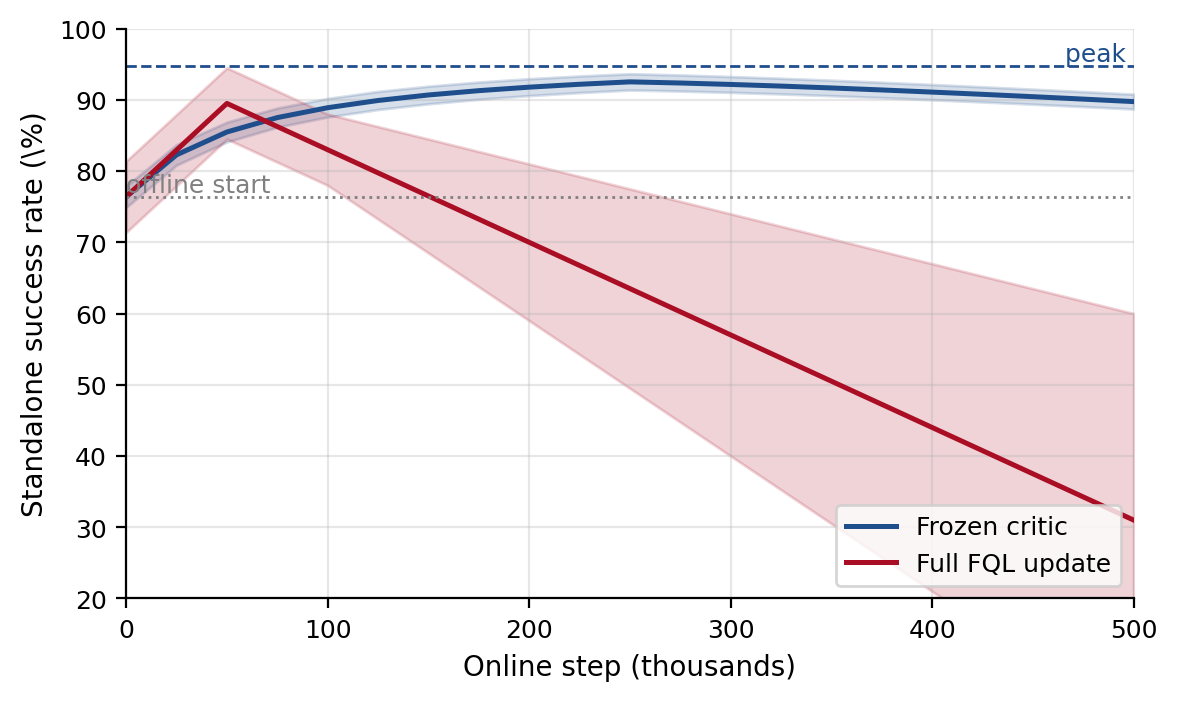
\includegraphics[width=0.85\linewidth]{figures/online_in_wm_curves.png}
\caption{Training trajectories for online fine-tuning inside the world
model. Both variants start from the same offline FQL checkpoint and use
the same FMQ-MPC planner to generate imagined transitions. Updating the
critic on imagined data leads to collapse after an early transient
improvement, whereas freezing the critic yields stable policy
improvement. Shaded regions show $\pm 1\sigma$ over three seeds.}
\label{fig:online-in-wm-curves}
\end{figure}

The final row of Table~\ref{tab:mpc-online-e2} applies the same FMQ-MPC
planner at test time on top of the best frozen-critic checkpoints. This
does not improve over the standalone actor peak
($93.2 \pm 0.7\%$ versus $94.8 \pm 0.7\%$). This suggests that the
actor has already absorbed most of the useful behaviour provided by the
planner during online fine-tuning. In other words, the world model has
served not as a reliable environment for critic learning, but as a
source of short-horizon policy-improvement supervision.
Thus, imagined transitions help only through an actor-only interface:
they provide useful policy-improvement data, but corrupt bootstrapped
value learning.

% ---------------------------------------------------------------------
\subsection{Goal-Conditioned Actor Fine-Tuning}
\label{sec:exp-mpc-online-wm-gc}

We now test the actor-only recipe in the full goal-conditioned setting
defined in \S\ref{sec:mpcd-gc}. The policy conditions on
$[z,z_{\mathrm{goal}}]$, training is shared across the five
\texttt{visual-cube-single} tasks, and rewards use the same
goal-conditioned indicator as offline pretraining. We compare direct
use of evaluation goals with achieved-state goals sampled from the
online buffer; the latter is the leakage-free protocol.

\begin{table}[h]
\centering
\caption{Goal-conditioned online fine-tuning inside the world model on
the five-task \texttt{visual-cube-single} benchmark. Success rate is
the standalone native OGBench success rate averaged over all five tasks
($50$ episodes per task), reported as mean $\pm$ standard deviation over
three seeds unless noted. The offline goal-conditioned baseline is
$90.0\%$.}
\label{tab:mpc-online-e3}
\begin{tabular}{llc}
\toprule
Online Training Variant & Goal Source & Final Success (\%) \\
\midrule
Offline goal-conditioned baseline & -- & 90.0 \\
\midrule
\multicolumn{3}{l}{\emph{Evaluation-goal training}} \\
HER relabelling, frozen critic & evaluation goals & 80.1 $\pm$ 1.6 \\
No HER relabelling, frozen critic & evaluation goals & 73.2 $\pm$ 1.2 \\
Mixed HER/no-HER (50/50), frozen critic & evaluation goals & 77.8 $\pm$ 3.0 \\
Mixed HER/no-HER (75/25), frozen critic & evaluation goals & 80.9 $\pm$ 1.5 \\
HER relabelling, updated critic & evaluation goals & 81.5 $\pm$ 1.3 \\
\midrule
\multicolumn{3}{l}{\emph{Achieved-state goal training}} \\
HER relabelling, frozen critic & achieved-state goals & 84.0 $\pm$ 1.5 \\
Mixed HER/no-HER (50/50), frozen critic & achieved-state goals & \textbf{84.4 $\pm$ 0.9} \\
\bottomrule
\end{tabular}
\end{table}

Table~\ref{tab:mpc-online-e3} shows that goal-conditioned
online-in-WM fine-tuning does not reliably improve over the offline
baseline. All final checkpoints fall below the $90.0\%$ offline policy,
including the variants that train directly on evaluation goals. The
strongest final results come from the leakage-free achieved-state
goal protocol: mixed HER/no-HER reaches $84.4 \pm 0.9\%$, and pure HER
reaches $84.0 \pm 1.5\%$. HER remains important, since the no-HER
evaluation-goal variant ends at only $73.2 \pm 1.2\%$.
The updated-critic row is also informative. Unlike the single-task
actor+critic update in Table~\ref{tab:mpc-online-e2}, it does not
collapse catastrophically: with the shared HIQL-style indicator reward,
updating the critic reaches $81.5 \pm 1.3\%$, close to the corresponding
frozen-critic evaluation-goal result of $80.1 \pm 1.6\%$. This supports
the interpretation that reward-scale mismatch was an important part of
the single-task critic-update failure, but it also shows that aligning
the reward scale is not sufficient to beat the offline baseline.
Unlike the single-task setting, freezing the critic is not sufficient to
produce a stable improvement. The likely reason is that the
goal-conditioned problem has substantially broader coverage
requirements. The actor must learn over the joint space
$(z,z_{\mathrm{goal}})$, and the online buffer generated by FMQ-MPC
covers only the narrow region visited by the current policy. As a
result, online fine-tuning tends to specialise the actor to the
distribution of imagined rollouts rather than improving performance
across the full benchmark.

% ---------------------------------------------------------------------
\subsection{Static World-Model Generated Dataset}
\label{sec:exp-wm-dataset-gen}

The previous experiments kept data generation coupled to the current
learner. We now evaluate the decoupled dataset-generation setting of
\S\ref{sec:mpcd-dataset-gen}: use the world model once to generate a
fixed synthetic corpus, then train offline RL methods without further
access to the model.

\paragraph{Setup.}
We compare three offline corpora, each containing approximately
$800$k goal-conditioned transitions across the five
\texttt{visual-cube-single} tasks:

\begin{itemize}
    \item \textbf{Real play data}: the original OGBench play dataset.
    \item \textbf{FMQ-generated data}: trajectories rolled out inside
    the world model using FMQ-MPC action selection
    ($N=32$, $H=2$, $\eta=0.02$).
    \item \textbf{BoN-generated data}: trajectories rolled out inside
    the world model using best-of-$N$ action selection without gradient
    refinement.
\end{itemize}

All corpora are stored without explicit goals: each transition contains
only latent states and actions, and goals are assigned during training
using the same HER sampler. This ensures that differences in downstream
performance come from the transition data itself, not from differences
in goal labelling.
We evaluate three downstream learners: FQL with a BC-flow actor, IQL
with AWR, and ReBRAC \cite{tarasov2023rebrac}. Performance is reported as the five-task native
success rate, averaged over three seeds.

\begin{table}[h]
\centering
\caption{Offline goal-conditioned learning from real and
world-model-generated corpora. Each corpus contains approximately
$800$k transitions and is processed with the same HER sampler during
training. \emph{Best Success} is the highest checkpoint over training;
\emph{Final Success} is the last checkpoint. Results are mean
$\pm$ standard deviation over three seeds.}
\label{tab:wm-dataset-gen}
\begin{tabular}{llrr}
\toprule
Learner & Training Corpus & Best Success (\%) & Final Success (\%) \\
\midrule
FQL (BC-flow actor) & Real play data & \textbf{90.3 $\pm$ 1.6} & 81.3 \\
FQL (BC-flow actor) & FMQ-generated data & 57.7 $\pm$ 3.8 & 41.7 \\
FQL (BC-flow actor) & BoN-generated data & 64.7 $\pm$ 3.7 & 55.7 \\
\midrule
IQL (AWR actor) & Real play data & 9.6 $\pm$ 1.8 & 5.3 \\
IQL (AWR actor) & FMQ-generated data & \textbf{16.4 $\pm$ 5.4} & 6.1 \\
IQL (AWR actor) & BoN-generated data & 16.0 $\pm$ 1.8 & 5.3 \\
\midrule
ReBRAC (TD3+BC actor) & Real play data & \textbf{13.7 $\pm$ 2.7} & 7.5 \\
ReBRAC (TD3+BC actor) & FMQ-generated data & 12.5 $\pm$ 3.4 & 5.7 \\
ReBRAC (TD3+BC actor) & BoN-generated data & 11.6 $\pm$ 1.4 & 6.7 \\
\bottomrule
\end{tabular}
\end{table}

Table~\ref{tab:wm-dataset-gen} shows that world-model-generated
datasets are substantially weaker than the original real play data for
the strongest downstream learner. FQL trained on real play reaches
$90.3 \pm 1.6\%$ best success, while the best synthetic corpus
(BoN-generated data) reaches only $64.7 \pm 3.7\%$. This gap persists
even though all corpora use the same HER procedure, indicating that the
limitation lies in the imagined trajectories themselves rather than in
the goal assignment process.
The comparison between FMQ-generated and BoN-generated data is also
informative. Although FMQ is the stronger online planner, it produces a
weaker offline dataset than BoN for FQL. This is because FMQ actions are
gradient-refined relative to the particular actor and critic used during
generation. When these actions are handed to a fresh learner, they no
longer arise from that learner's own policy distribution and are harder
to imitate. By contrast, BoN actions are unmodified samples from the
flow actor, making them more natural targets for a new flow-matching
policy.
The weaker performance of IQL and ReBRAC is less informative about the
datasets themselves. Both methods perform poorly across all corpora,
including real play data, suggesting that their policy classes and
training objectives struggle with the high-dimensional action chunks in
this benchmark. FQL is therefore the clearest indicator of corpus
quality.
Overall, the world model is not an adequate one-shot replacement for
real offline data. The useful signal in earlier sections depends on the
closed loop between the current actor, planner, and critic; once a fixed
synthetic corpus is handed to a fresh learner, much of that benefit is
lost.

% ---------------------------------------------------------------------
\section{World Model as Data Generator for New Environments}
\label{sec:exp-generalisation}

We next ask whether online-in-WM generalises beyond
\texttt{cube-single}. We evaluate two additional OGBench domains:
\texttt{visual-scene-play-v0}, which contains object-placement tasks in
a cluttered scene, and \texttt{visual-puzzle-3x3-play-v0}, which
contains button-configuration tasks on a $3\times3$ puzzle. In both
cases, a separate LeWM world model is trained from the corresponding
play dataset.

The key diagnostic is the \emph{action-conditioning ratio}: the factor
by which prediction error increases when the action sequence is
shuffled. High ratios indicate a steerable model; ratios near $1.0$
indicate that MPC has little basis for distinguishing action sequences.

\subsection{Action Conditioning as a Generalisation Diagnostic}
\label{sec:exp-gen-wm}

Before running the full RL pipeline, we measure the action-conditioning
ratio for each environment. This diagnostic is cheap to compute from
the latent cache and does not require pixel re-rendering or policy
training.

\begin{table}[h]
\centering
\caption{Action-conditioning ratio across environments. The ratio
measures how much prediction error increases when actions are shuffled
relative to the true action sequence. Larger values indicate that the
world model is more strongly action-conditioned and therefore more
suitable for MPC-based control.}
\label{tab:action-conditioning}
\begin{tabular}{lcc}
\toprule
Environment & Action-conditioning ratio & Expected online-in-WM effect \\
\midrule
\texttt{cube-single} & $8.0\times$ & strong improvement \\
\texttt{scene} & $1.4\times$ & small or marginal improvement \\
\texttt{puzzle-3x3} & $1.1\times$ & weak or harmful effect \\
\bottomrule
\end{tabular}
\end{table}

Table~\ref{tab:action-conditioning} shows that the three environments
span a wide range of action sensitivity. The cube environment has a
strongly action-conditioned world model, which is consistent with the
large gains observed earlier. In contrast, the scene and puzzle models
are only weakly action-conditioned. This suggests that MPC rollouts in
these environments may not reliably distinguish good actions from bad
ones, limiting the effectiveness of online-in-WM.
The remainder of this section tests whether this diagnostic predicts
the downstream RL results.

\subsection{Single-Task Online-in-WM}
\label{sec:exp-gen-single-task}

We first evaluate the single-task version of online-in-WM, matching the
protocol of \S\ref{sec:exp-mpc-online-wm}. The agent is trained for
$500$k FMQ-MPC steps inside the world model, using a frozen critic and
standalone evaluation without a planner at test time.

\begin{table}[h]
\centering
\caption{Single-task online-in-WM generalisation results. The method is
the frozen-critic online-in-WM procedure from
\S\ref{sec:exp-mpc-online-wm}, evaluated on task 1 of each environment.
Success is measured without a planner at test time over $250$
episodes.}
\label{tab:gen-single-task}
\begin{tabular}{lccc}
\toprule
Environment & Offline Success (\%) & Final Success (\%) & Peak Success (\%) \\
\midrule
\texttt{scene} & 18.8 & $17.1 \pm 2.4$ & $20.4 \pm 1.2$ \\
\texttt{puzzle-3x3} & 44.4 & 50.4 & 54.0 \\
\bottomrule
\end{tabular}
\end{table}

Table~\ref{tab:gen-single-task} reports these results. For \texttt{scene},
online-in-WM provides at most a marginal improvement. The peak success rate rises from $18.8\%$ to
$20.4 \pm 1.2\%$, but the final checkpoint falls slightly below the
offline baseline. This is consistent with the weak
$1.4\times$ action-conditioning ratio: the world model contains some
action information, but not enough to support strong policy
improvement.
The \texttt{puzzle-3x3} result is numerically positive, reaching
$54.0\%$ peak success from a $44.4\%$ offline baseline. However, this
environment has an action-conditioning ratio of only $1.1\times$, so
the result should be interpreted cautiously. The world model is nearly
action-agnostic, and the online curve is correspondingly high variance.
The result is therefore best viewed as a weak positive signal rather
than strong evidence of robust generalisation.
Overall, the single-task results are much weaker than those observed on
\texttt{cube-single}. This already suggests that online-in-WM depends
strongly on the steerability of the learned dynamics model.

\subsection{Goal-Conditioned Online-in-WM}
\label{sec:exp-gen-goal-conditioned}

We next evaluate the full goal-conditioned setting. This is the harder
test: the policy must generalise across all five tasks, conditions on
both the current latent state and the goal latent, and uses HER during
online fine-tuning. The protocol matches
\S\ref{sec:exp-mpc-online-wm-gc}.

\begin{table}[h]
\centering
\caption{Goal-conditioned online-in-WM generalisation results.
Performance is averaged across all five tasks, with $50$ evaluation
episodes per task. Success is measured without a planner at test time.}
\label{tab:gen-goal-conditioned}
\begin{tabular}{lccc}
\toprule
Environment & Offline Success (\%) & Final Success (\%) & Peak Success (\%) \\
\midrule
\texttt{scene} & 8.4 & $8.4 \pm 0.6$ & $10.7 \pm 1.0$ \\
\texttt{puzzle-3x3} & 3.2 & 0.8 & 3.6 \\
\bottomrule
\end{tabular}
\end{table}

Table~\ref{tab:gen-goal-conditioned} reports the goal-conditioned results,
which are weaker than the single-task results.
For \texttt{scene}, online-in-WM matches the offline baseline at the
final checkpoint and reaches only a small peak improvement of
$10.7 \pm 1.0\%$. For \texttt{puzzle-3x3}, performance decreases:
the final success rate falls from $3.2\%$ to $0.8\%$, and the best
checkpoint only recovers to $3.6\%$.
The per-task breakdown in Table~\ref{tab:gen-goal-conditioned-tasks}
shows why the five-task average remains low. In both environments,
non-zero success is concentrated almost entirely on task 1, while tasks
2--5 remain unsolved. The online-in-WM phase therefore does not
discover broad goal-conditioned competence; it mainly reinforces the
easiest part of the task distribution.

\begin{table}[h]
\centering
\caption{Per-task final success rates for goal-conditioned
online-in-WM. Success is concentrated on task 1; tasks 2--5 remain at
$0\%$ throughout training in both environments.}
\label{tab:gen-goal-conditioned-tasks}
\begin{tabular}{lrrrrrr}
\toprule
Environment & Task 1 & Task 2 & Task 3 & Task 4 & Task 5 & Average \\
\midrule
\texttt{scene} & $\sim 41.0$ & 0.0 & 0.0 & 0.0 & 0.0 & 8.4 \\
\texttt{puzzle-3x3} & 4.0 & 0.0 & 0.0 & 0.0 & 0.0 & 0.8 \\
\bottomrule
\end{tabular}
\end{table}

These results indicate that the goal-conditioned setting is more
sensitive to weak action conditioning than the single-task setting. The
policy must cover a larger input space, since observations contain both
the current latent state and the goal latent. In addition, successful
online updates require the MPC controller to generate transitions that
move specifically toward the requested goal, not merely plausible
transitions under the world model. When the predictor is weakly
action-conditioned, imagined rollouts do not reliably reflect
goal-directed consequences of actions, and the generated buffer becomes
too noisy to improve the policy.

\paragraph{Summary.}
The three-environment comparison points to a simple regularity:
action conditioning appears to be necessary for online-in-WM to work.
On \texttt{cube-single}, where the action-conditioning ratio is
$8.0\times$, the method produces a large improvement. On
\texttt{scene}, where the ratio is only $1.4\times$, gains are small.
On \texttt{puzzle-3x3}, where the ratio is $1.1\times$, the
goal-conditioned method is ineffective or harmful.
This diagnostic is useful because it can be computed cheaply before
running the full RL pipeline. In practice, it provides a screening test
for whether a learned world model is likely to be steerable enough to
support MPC-based online fine-tuning.

% ---------------------------------------------------------------------
\section{Latent Subgoal Planning Results}
\label{sec:exp-wm-as-subgoal}

The final experiments evaluate Latent Subgoal Planning (LSP), introduced
in Chapter~\ref{chap:wm-as-subgoal}. LSP uses the world model at the
high level: Phase 1 trains a purely offline hierarchy, while Phase 2
freezes the low-level controller and value function and updates only
the high-level subgoal policy.

\subsection{Offline Hierarchical Baseline}
\label{sec:exp-lsp-phase1}

Phase 1 establishes the offline LSP baseline. It replaces the Gaussian
high- and low-level policies of HIQL with flow-matching actors, but uses
no world-model rollouts during training.

\begin{table}[h]
\centering
\caption{Offline hierarchical baseline on OGBench
\texttt{cube-single}. LSP Phase 1 replaces the Gaussian high- and
low-level policies of HIQL with flow-matching policies while remaining
purely offline. Success rate is the native five-task average.}
\label{tab:lsp-phase1}
\begin{tabular}{lr}
\toprule
Method & Success (\%) \\
\midrule
HIQL end-to-end & 87.0 \\
LSP Phase 1 (flow HL + flow LL) & \textbf{88.0} \\
\bottomrule
\end{tabular}
\end{table}

Table~\ref{tab:lsp-phase1} shows that the Phase-1 LSP baseline is
already competitive with end-to-end HIQL, slightly improving the
five-task average from $87.0\%$ to $88.0\%$. The remaining experiments
therefore test whether the world model can improve an already strong
offline hierarchy, rather than rescuing a weak baseline.

\subsection{World-Model-Grounded AWR}
\label{sec:exp-phase2-awr}

Table~\ref{tab:lsp-phase2-awr} evaluates the Phase-2 AWR update from
\S\ref{sec:lsp-awr-data}, sweeping the temperature $\alpha$. The frozen
high-level control checks whether Phase-1 performance is preserved, and
the offline AWR control isolates the effect of the high-level update
from world-model rollout error.

\begin{table}[h]
\centering
\caption{Phase-2 high-level AWR updates on OGBench
\texttt{cube-single}. Step-0 is the Phase-1 checkpoint at the start of
Phase 2. Peak is the best evaluation checkpoint, and final is the
checkpoint after $500{,}000$ updates. All runs freeze the low-level
policy.}
\label{tab:lsp-phase2-awr}
\begin{tabular}{llrrr}
\toprule
Update Type & $\alpha$ & Step-0 (\%) & Peak (\%) & Final (\%) \\
\midrule
No high-level update & --  & 85 & 89 & 87 \\
\midrule
World-model AWR & 5.0  & 77 & 88 & 79 \\
World-model AWR & 2.0  & 82 & 84 & 76 \\
World-model AWR & 1.0  & 83 & 71 & 54 \\
World-model AWR & 0.5  & 80 & 39 & 29 \\
World-model AWR & 0.1  & 88 & 12 & 6 \\
\midrule
Offline AWR control & 2.0  & 81 & 92 & 63 \\
Offline AWR control & 1.0  & 83 & 73 & 60 \\
Offline AWR control & 0.1  & 80 & 15 & 6 \\
\bottomrule
\end{tabular}
\end{table}

The frozen high-level control preserves performance, ending at
$87\%$. This confirms that degradation is not caused by the evaluation
protocol; it appears only when
the high-level policy is updated.
The world-model AWR rows show no reliable improvement over Phase 1.
At high temperature ($\alpha=5.0$), the update is highly selective and
performance is mostly preserved, reaching $88\%$ peak but falling to
$79\%$ final. As $\alpha$ decreases, the update spreads probability mass
over a broader set of subgoal targets and performance degrades rapidly,
collapsing to $6\%$ final at $\alpha=0.1$.
The offline AWR control shows the same pattern. Even without world-model
rollouts, updating the high-level flow policy toward broad dataset
subgoal targets destabilises the hierarchy. The $\alpha=2.0$ offline
control briefly reaches $92\%$, but this is not stable and falls to
$63\%$ by the final checkpoint. This suggests that the core failure is
not simply inaccurate world-model evaluation. Instead, the high-level
AWR update changes the subgoal distribution in a way that the frozen
low-level policy cannot reliably follow. In effect, the update
de-sharpens a strong Phase-1 high-level policy rather than improving it.

\subsection{AWR with Achieved Latent States}
\label{sec:exp-phase2-hrf}

Table~\ref{tab:lsp-hrf} evaluates Hindsight Reality Forcing (HRF), the
achieved-state variant introduced in \S\ref{sec:lsp-hrf}. HRF tests
whether replacing proposed subgoals with rollout endpoints avoids the
value-gaming failure mode of AWR.

\begin{table}[h]
\centering
\caption{Phase-2 Hindsight Reality Forcing (HRF). Step-0 is the
Phase-1 baseline. HRF replaces proposed-subgoal targets with the latent
states achieved after world-model rollouts.}
\label{tab:lsp-hrf}
\begin{tabular}{llrrrr}
\toprule
Update Type & Low-Level Policy & Step-0 (\%) & 50k (\%) & 100k (\%) & 500k (\%) \\
\midrule
HRF, $\alpha=1.0$ & frozen  & 82 & 0 & 0 & 0 \\
HRF, $\alpha=3.0$ & frozen  & 88 & 0 & 1 & 0 \\
HRF, $\alpha=1.0$ & updated & 80 & 0 & 0 & 0 \\
\bottomrule
\end{tabular}
\end{table}

HRF fails immediately. All configurations collapse to approximately
zero success by the first evaluation checkpoint at $50$k steps. This
shows that the problem is not only value gaming. Even when the update
is forced to imitate the achieved rollout endpoint, the resulting
targets occupy a distribution that differs from the dataset subgoals on
which the low-level policy was trained.
Updating the low-level policy alongside the high-level policy does not
solve the issue. Once the high-level distribution shifts, the low-level
targets shift with it, and the hierarchy loses the coordination learned
during Phase 1.
The LSP experiments are therefore a negative result. Phase 1 gives a
strong offline hierarchy, but both AWR and HRF destabilise it once the
high-level subgoal distribution shifts away from the distribution on
which the low-level policy was trained.
Further Phase-2 ablations --- the low-level reachability metric,
low-level freezing, high-level update cadence, and an alternative
real-candidate grounding mode --- are reported in
Appendix~\ref{app:lsp-ablations}.

% ---------------------------------------------------------------------
\section{Headline Results and Empirical Findings}
\label{sec:exp-headline}

This section collects the main empirical results and the two findings
that explain the overall pattern.

\begin{table}[h]
\centering
\caption{Headline comparison across the main experimental settings.
Single-task results are evaluated on
\texttt{visual-cube-single-singletask-task1-v0} over $250$ episodes.
Goal-conditioned results are five-task native OGBench averages. The
table reports the best representative result for each method family.}
\label{tab:headline}
\begin{tabular}{llc}
\toprule
Method & Setting & Success (\%) \\
\midrule
\multicolumn{3}{l}{\emph{Offline and non-WM baselines}} \\
Offline FQL checkpoint & single-task & 81.6 \\
Q-chunking reference & single-task & 92.8 \\
HIQL end-to-end & goal-conditioned, 5 tasks & 87.0 \\
\midrule
\multicolumn{3}{l}{\emph{World model as a training environment}} \\
World Model RL (Sparse Reward, 3 seeds) & single-task & $24.5 \pm 5.1$ \\
Anchored World Model RL (Dense Reward) & single-task & 15.2 \\
Joint Predictor--Policy Training & single-task & 9.6 \\
Nearest-Neighbour Regularisation & single-task & 2.4 \\
\midrule
\multicolumn{3}{l}{\emph{Inference-time planning with a frozen policy}} \\
BoN-MPC, $H=1$ & single-task & 88.0 \\
Grad-MPC, $H=2$, $K=5$ & single-task & 90.0 \\
FMQ on frozen critic, $\eta=0.1$ & single-task & 90.0 \\
\midrule
\multicolumn{3}{l}{\emph{Policy learning from MPC-generated data and calibrated inference}} \\
Grad-MPC interleaved training, critic-update setting & single-task & 92.4 \\
FMQ-trained actor + FMQ inference & single-task & \textbf{96.0} \\
FMQ-trained actor + Grad-MPC inference, $K=8$ & single-task & \textbf{96.0} \\
\midrule
\multicolumn{3}{l}{\emph{Online fine-tuning inside the world model}} \\
Online-in-WM, actor+critic update & single-task & 30.7 $\pm$ 20.8 \\
Online-in-WM, frozen critic (final) & single-task & 90.7 $\pm$ 0.8 \\
Online-in-WM, frozen critic (peak) & single-task & \textbf{94.8 $\pm$ 0.7} \\
Goal-conditioned online-in-WM, achieved-state goals (final) & goal-conditioned, 5 tasks & 84.4 $\pm$ 0.9 \\
\midrule
\multicolumn{3}{l}{\emph{Latent Subgoal Planning}} \\
LSP Phase 1 (flow HL + flow LL) & goal-conditioned, 5 tasks & \textbf{88.0} \\
LSP Phase 2, World-model AWR, best final & goal-conditioned, 5 tasks & 79.0 \\
LSP Phase 2, Hindsight Reality Forcing & goal-conditioned, 5 tasks & $\approx 0$ \\
\midrule
\multicolumn{3}{l}{\emph{Generalisation to new environments}} \\
Single-task online-in-WM, \texttt{scene}  & single-task & 20.4 $\pm$ 1.2 \\
Single-task online-in-WM, \texttt{puzzle-3x3} & single-task & 54.0 \\
Goal-conditioned online-in-WM, \texttt{scene}  & goal-conditioned, 5 tasks & 10.7 $\pm$ 1.0 \\
Goal-conditioned online-in-WM, \texttt{puzzle-3x3} & goal-conditioned, 5 tasks & 3.6 \\
\bottomrule
\end{tabular}
\end{table}

Table~\ref{tab:headline} shows the main pattern. The weakest results
come from treating the world model as a replacement environment; the
strongest single-task results come from local planning,
planner-generated action supervision, and actor-only online-in-WM. The
goal-conditioned results are more limited: LSP Phase 1 is the strongest
stable five-task method, but Phase 2 world-model updates and
goal-conditioned online-in-WM do not reliably beat the offline
baselines.

\paragraph{Finding 1: the offline critic is the most reliable bridge
between imagined rollouts and real task success.}
The most successful methods use LeWM to generate candidate futures and
the offline critic to choose among them. This matters because the critic
is better aligned with native task success than latent distance alone:
CEM reaches the goal embedding with $0.0\%$ native success, whereas
BoN-MPC, Grad-MPC, and FMQ improve by ranking candidates with the
real-data critic. Once imagined successors enter Bellman targets,
however, prediction error can corrupt the critic itself.

\paragraph{Finding 2: world models are useful locally, but unreliable
as long-horizon training environments.}
One- and two-step planning improves performance, and gradient-based
action refinement provides additional gains. Longer imagined training
loops are much less reliable: prediction drift corrupts value learning,
static synthetic corpora underperform real play data, and Phase-2 LSP
updates create a subgoal distribution shift that the frozen low-level
policy cannot absorb. The consistent positive case is therefore local:
LeWM proposes short-horizon improvements, the offline critic selects
among them, and the actor absorbs the improvement without rewriting the
value function.

% ---------------------------------------------------------------------
\section{Limitations and Threats to Validity}
\label{sec:exp-threats}

The results in this chapter give a consistent picture, but they should
not be read as a complete statement about all latent world models or all
offline RL settings. The strongest single-task results come from one
OGBench domain, and each environment is evaluated with one frozen LeWM
checkpoint. The cross-environment experiments in
\S\ref{sec:exp-generalisation} make this less narrow by testing where
the recipe transfers, but they do not remove the dependence on the
particular model family used here. A world model with different training
data, architecture, or long-horizon accuracy could change where the
boundary lies between useful short-horizon prediction and harmful model
exploitation.

The experimental coverage is also uneven. The online-in-WM comparisons
use three or four seeds, but several inference-time MPC sweeps
(Tables~\ref{tab:mpc-bon}--\ref{tab:mpc-fmq-distilled}) and the LSP
Phase-2 experiments are single runs evaluated over many episodes. The
$96.0\%$ result is also the best checkpoint from a sweep, so it is best
viewed as evidence that the method can reach that level, not as a fully
seeded estimate of its expected performance. This is why final
checkpoints are reported alongside peak checkpoints where possible:
final performance is the fairer measure when no real-environment
validation signal should be available during deployment.

Comparisons with external baselines should be interpreted with similar
care. The methods in this thesis were tuned through the sweeps in
Appendix~\ref{app:oo-sweeps}, while the Q-chunking reference value of
$92.8\%$ is a published number obtained under a separate tuning budget.
The comparison is still useful as a reference point, but the margin over
Q-chunking should not be treated as a perfectly controlled benchmark
comparison.

There is also a leakage issue in some of the goal-conditioned
experiments. Variants that train directly on evaluation goals are useful
diagnostics, because they show what happens when the intended goal
distribution is given to the online-in-WM loop. They are not, however,
the cleanest protocol. For that reason, the achieved-state goal results
in \S\ref{sec:exp-mpc-online-wm-gc} are the main leakage-free numbers,
and the conclusions about goal-conditioned online-in-WM are based on
those results.

Finally, the most successful online-in-WM method relies heavily on the
offline critic. The same critic scores MPC candidates and provides the
training signal for the actor, so any systematic critic error could be
reinforced rather than corrected. The real-environment gains suggest
that this was not the dominant failure mode on the benchmarks studied,
but the method still depends on the critic being better grounded than
the world model predictions it evaluates.
